\section{Simulations}
\subsection{Implementation on Matlab}
We will now discuss the technical details of the implementation used for simulating the robot. We used Simulink as our main simulator for this project. The 3R rigid robot has been implemented using a Matlab function block that computes the direct dynamics followed by two integrators. To turn this into an elastic joint robot, we put a block that takes care of the spring coupling between motor and link by exchanging elastic forces between \(q\) and \(\theta\). To implement the iterative control law, we crafted a \textbf{sample and hold} block Figure~\ref{sandh} which samples the input only when a certain boolean signal has a rising edge. This has been used to update the terms \(u_i\) and \(\theta_{d,i}\) in the control law. The update condition was first set to a threshold on \(\dot \theta\) to detect the steady state:
\[
    upd : \| \dot \theta \| < thr = 10^{-3}
\]
This worked quite well on the rigid robot but far less on the elastic joint one, as a matter of facts in most experiments this condition was never met, resulting in no iterations. This is caused by the high frequency oscillations in the model that never let the velocities cancel. This behavior arises from the fact that we did not model any kind of dissipation in the robot, particularly by including relative spring damping \(D\dot \delta\) those oscillations would automatically dampen. Another possible solution is to perform the update at certain time steps where you assume the robot had enough time to reach an approximate steady state; this way, the quantities updated are estimated (i.e. \(u_i \neq g(q_i) \)) but in practice we have found that despite this the robot reaches the desired configuration, the fastest results are attained when the conditions are in or.

\begin{figure}[h!]
\centerline{\includegraphics[scale=0.5]{figures/sampleandhold.png}}
\caption{\label{sandh}
The Sample\&Hold block used in our controllers, exploiting boolean logic it's possible to output the correct signal during each iteration.}
\end{figure}
\subsection{Experiments}
We've carried out some experiments testing the performance of the iterative controller with various cases of stiffness down to very soft joints, while keeping constant the other robot parameters: the links have equal length \textit{l = 1 m}, with uniformly distributed masses \textit{m1, m2, m3 of 10, 7.5, and 5 kg} respectively. We've also tried different gain matrices to understand how much the sufficient assumptions could be relaxed. Using a random sampling of the q space we have been able to estimate $\alpha$ \textit{= 340}.
\subsubsection{High rigidity}
To validate our script we started using the huge levels of rigidity we found in \cite{simplepd}: $K_1 = 14210, K_2 = 29800, K_3 = 13500 ~~Nmrad^{-1}$, in this situation it is possible to play with $\gamma$ and $\beta $ in such a way that the gains are not very high while completely satisfying the convergence assumptions. Being into the bounds even when $\gamma = 35$, it's possible to set $\beta = 0.47$ and with $K_p = diag\{600, 500, 400\},  K_d=diag\{200,200,200\}$ we got amazing results for all our trials. We see them in our first experiment that consist in reaching $q_d=(\pi/4,0,\pi/2)$ from $q_0=(-\pi/2,0,0)$ at rest: Figures~\ref{1_1err}\&\ref{1_1ceff} show the errors and the applied torques (control effort) over 12 seconds, with a new iteration each 3 seconds only four are needed to converge. It is interesting to note how in Figure~\ref{1_1qt} there is nearly no displacement between q and theta, indeed as we said this is a feature of elastic joint robots and we are in a situation where it's hard to spot the difference with rigid case, in a certain sense we are using the same method validated for that kind of robots but with stronger assumption so one can expect to do very well.
\begin{figure}[h!]
\centerline{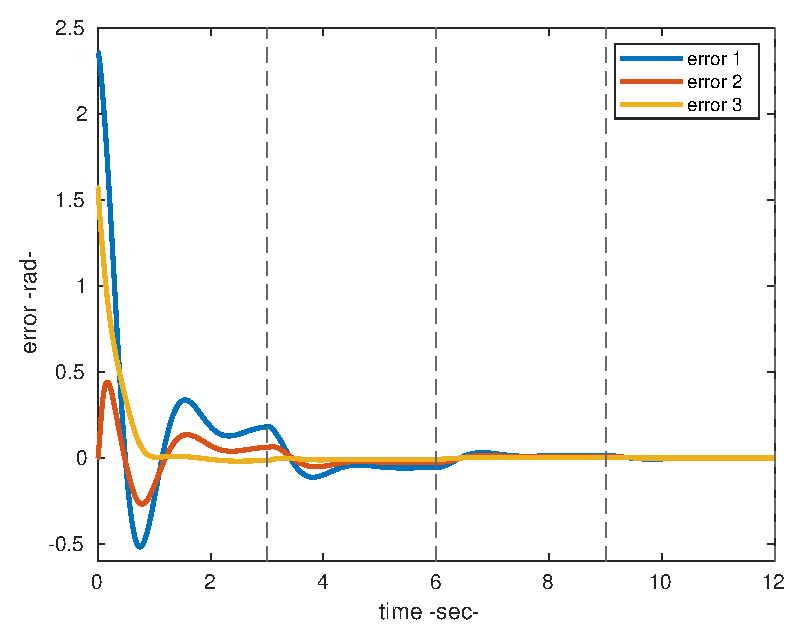
\includegraphics[scale=0.42]{figures/1_1_error.eps}}
\caption{\label{1_1err}
Experiment 1: joint level error.}
\end{figure}

\begin{figure}[h!]
\centerline{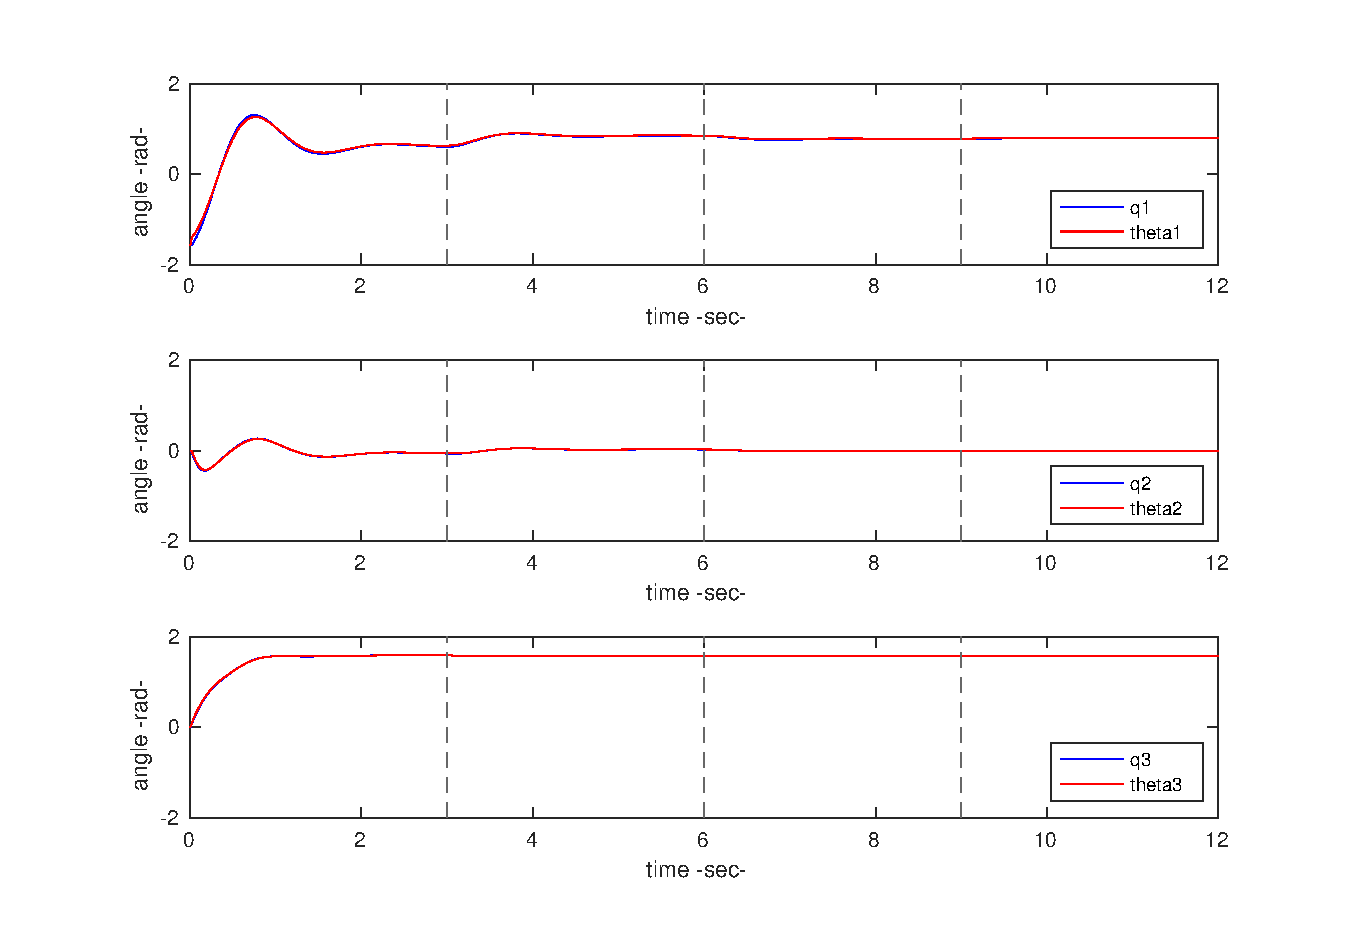
\includegraphics[scale=0.42]{figures/1_1_qtheta.eps}}
\caption{\label{1_1qt}
Experiment 1: q and \(\theta\) evolution.}
\end{figure}

\begin{figure}[h!]
\centerline{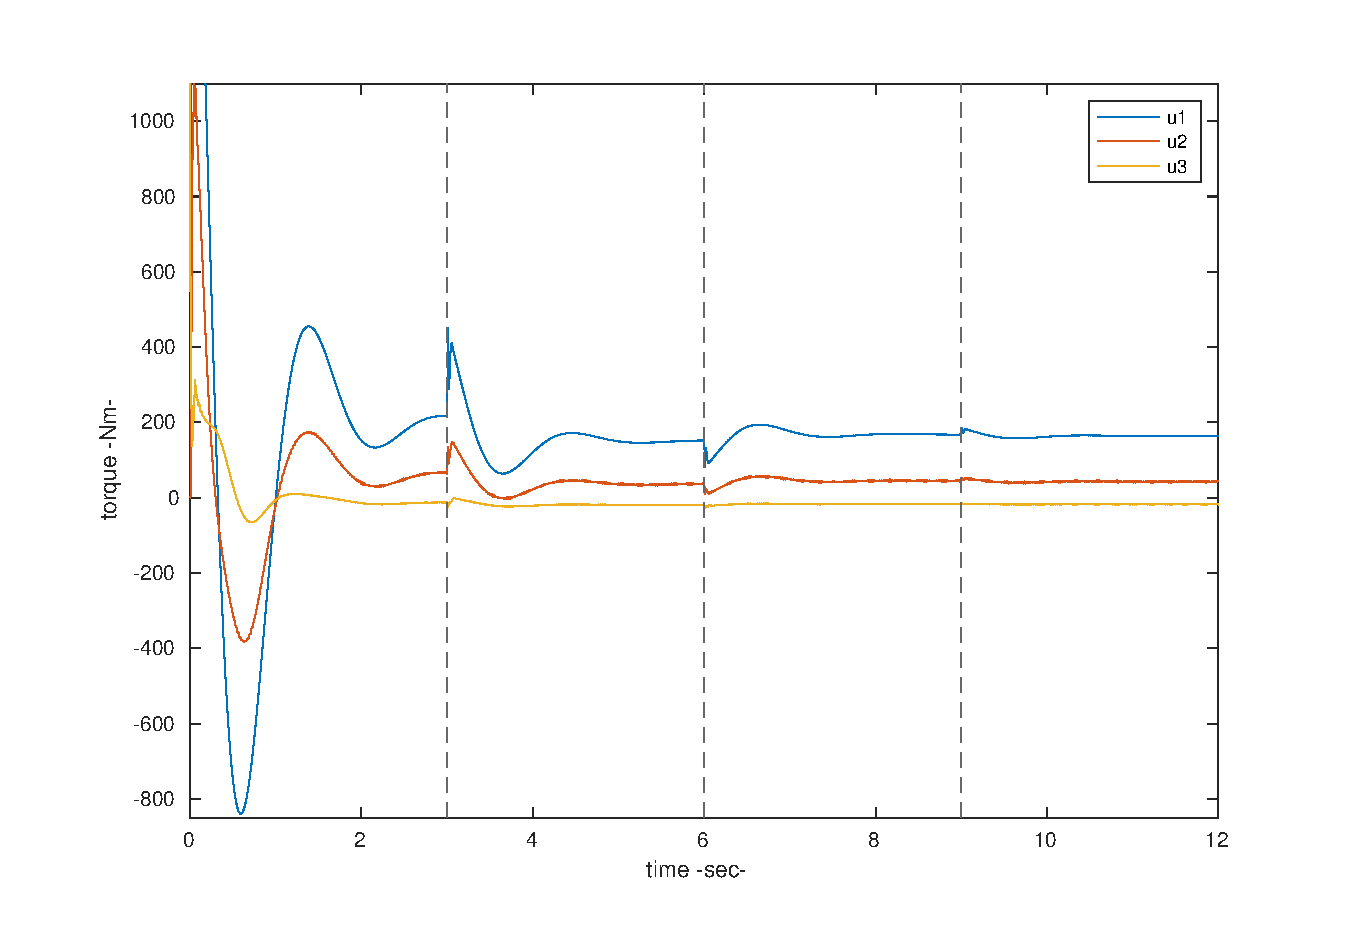
\includegraphics[scale=0.42]{figures/1_1_ceffort.eps}}
\caption{\label{1_1ceff}
Experiment 1: applied torque.}
\end{figure}
\clearpage
\subsubsection{Medium rigidity}
After that, to get meaningful results we considerably scale down the stiffness to what we call "medium value" according to our investigations: $K_1 = 2100, K_2 = 4500, K_3 = 1500 ~~Nmrad^{-1}$. Setting $\gamma = 5, \beta = 0.3$, we've configured the control with very low gains $K_p = diag\{200, 200, 200\}, K_d=diag\{150,150,150\}$. As one can expect the convergence will be slower, but it's not the only problem; we are not satisfying many assumption of the theorem: a) due to $K_3$ and b) due to the fact that each element of $K_p$ is lower than \(\alpha\). Nevertheless, as it's possible to see in Figures~\ref{2_1err}\&\ref{2_2err} we are performing very well both on Experiment 2 (which is aiming to get the same desired configuration of experiment1) and Experiment 3 (which want to bring the arm in $q_d=(0,0,0)$ from the same initial conditions of experiment 2). This suggest for example that in c) $\beta$ is not "strictly" constrained and, in general, stress out how a)-d) are not necessary conditions.  
However, 3 seconds step iteration regardless of the robot’ state, requires seven updates for Exp. 2 and five for Exp. 3. In these cases is much easier to identify the displacement from Figures~\ref{2_1qt}\&\ref{2_2qt} since the elasticity is not negligible.
In order to complete this analysis we show how in Exp. 2 (very similar results apply to all the success case) the control term converges to the gravity one in the desired configuration Figure~\ref{2_1gravff} and how slowly $\theta_d$ departs from $q_d$ as the time pass Figure~\ref{2_1tqd}. Lastly, if one is curious to verify which is the steady state error of the simple PD controller in Figure~\ref{2_1pdvit} we even compare its performance with the iterative method assuring to have the same $K_p$, indeed we have same behaviour before the first update.

\subsubsection{Low rigidity}
To test the limits of the iterative controller we further soften the stiffness to the values: $K_1 = 1500, K_2 = 1000, K_3 = 500 ~~Nmrad^{-1}$. With these parameters we violate the conditions of convergence, event with the smallest possible value of \(\gamma\) which is \(2\). As a result, we get a very small number for \(\beta = \frac{1}{400}\). Since our proportional gain is divided by theta, we have to set it very low to avoid unwanted oscillations. In this experiment (from $q_0=(-\pi/2,0,0)$ to $q_d=(\pi/4,0,\pi/2)$) we have set $K_p = diag\{7.5, 5, 0.75\}, K_d=diag\{2000,1000,800\}$. The small proportional gains do not satisfy condition c) of the convergence proof. The high derivative gain values are justified by the fact that we want to excite as less oscillations as possible on motor positions while slowly moving them to \(\theta_d\), in order to keep link positions close to motor positions. Here we do not have perfect convergence, but we get very close after 4 iterations with just oscillations around \(q_d\) which have a very small amplitude of \(0.03 rad\) Figure \ref{4_e}. By lowering \(K_d\) to \(diag\{200,200,200\}\) we do not get convergence at all, and a oscillation behavior arises on \(\theta\), which makes it very difficult to stop the oscillations on the link position. This also translates in very bad joint torque profiles Figure \ref{5_u}.
\begin{center}
\begin{figure}[h!]
\begin{minipage}[h!]{0.45\linewidth}
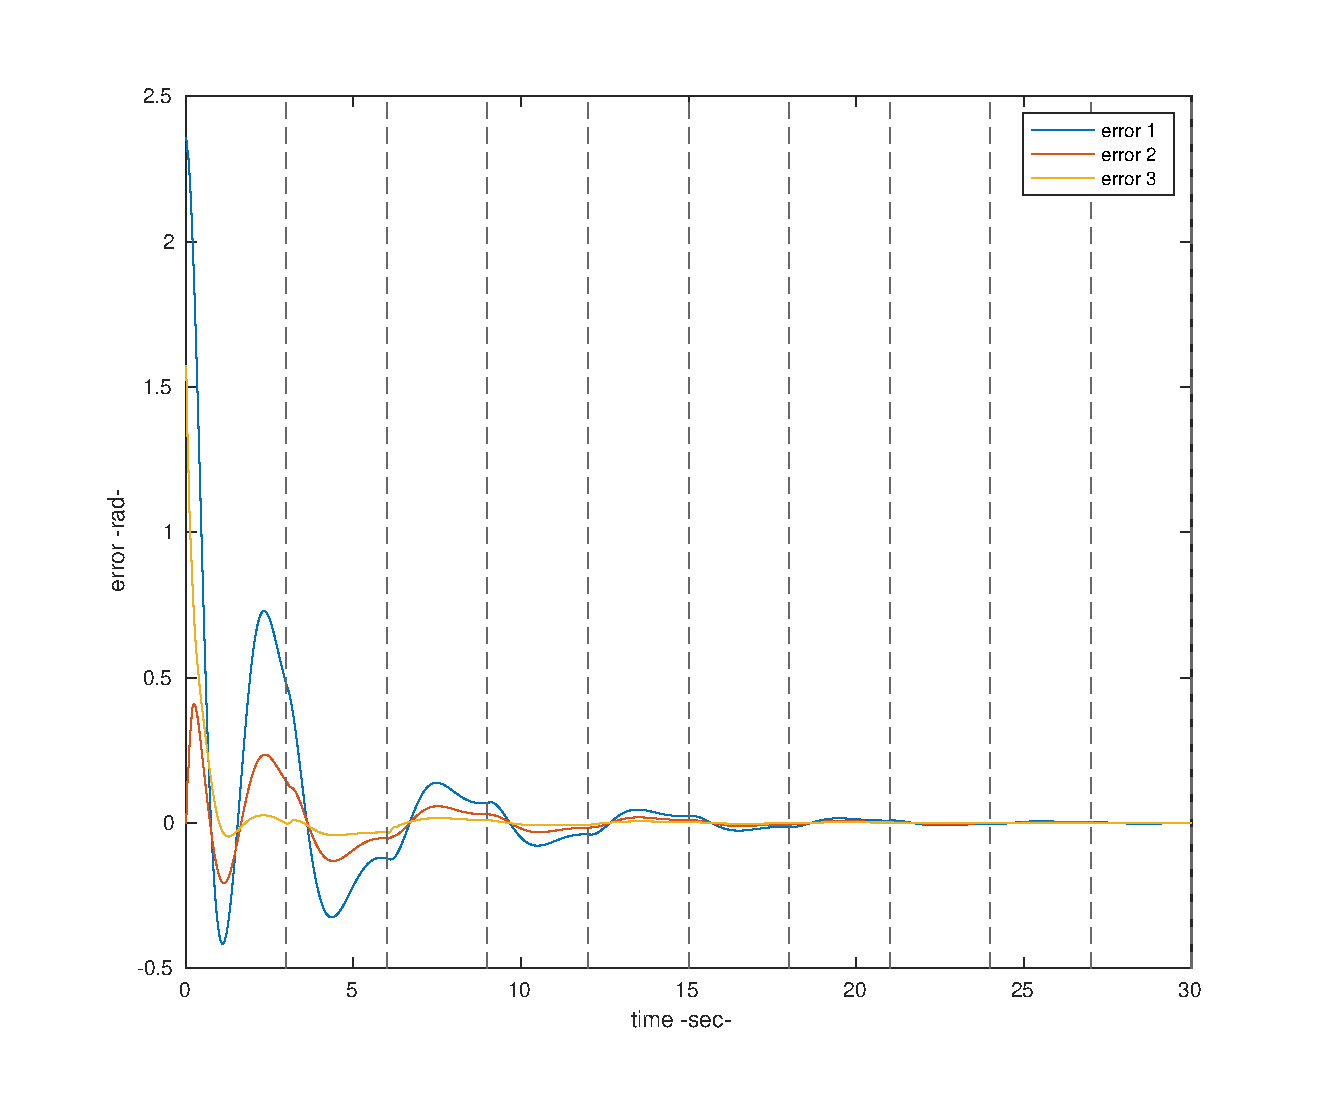
\includegraphics[scale=0.35]{figures/2_1_error.eps}
\caption{\label{2_1err}
Exp. 2: joint level error.}
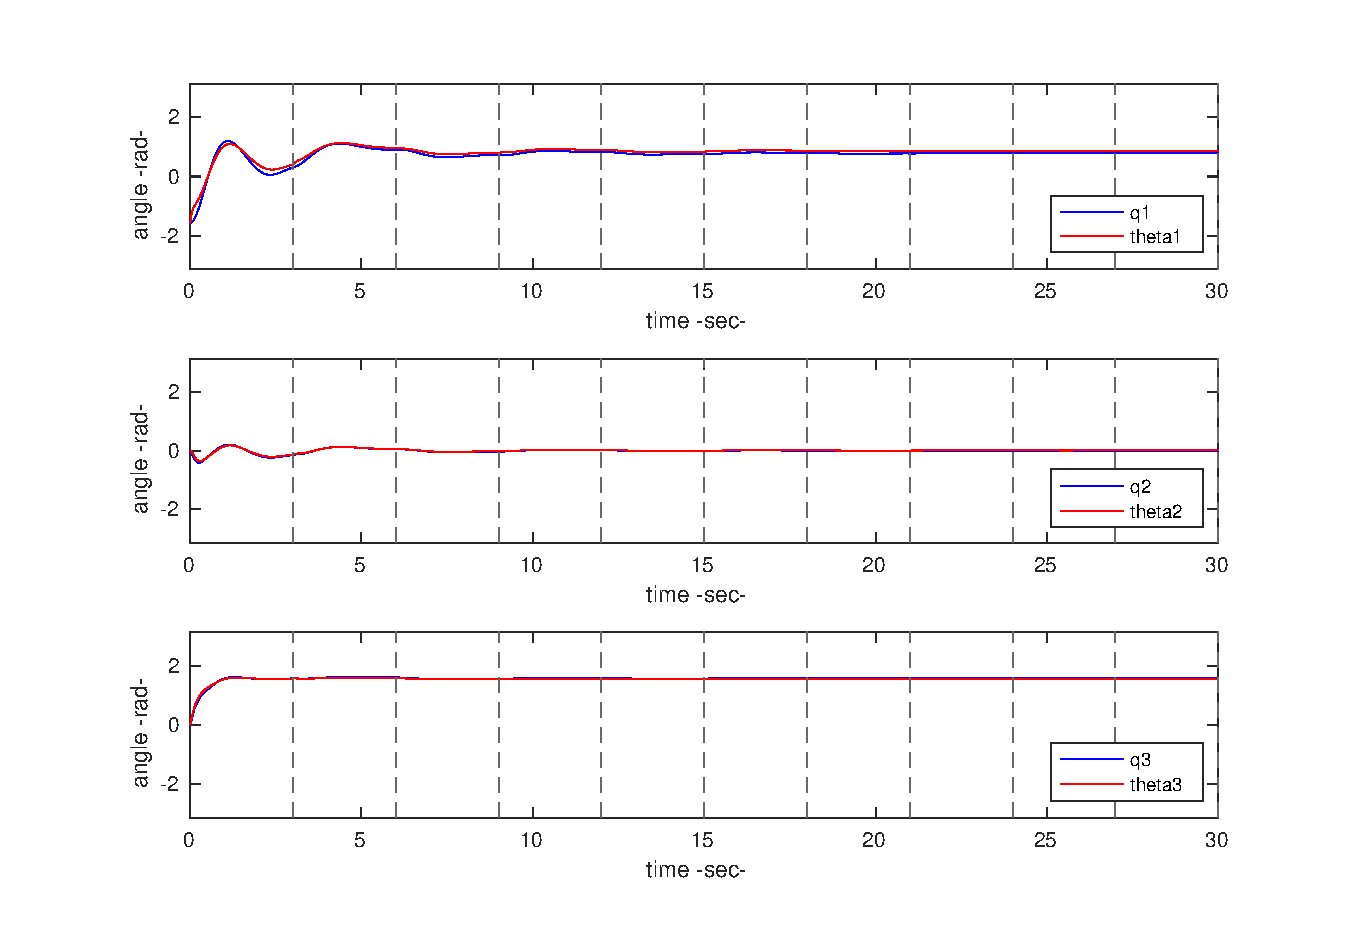
\includegraphics[scale=0.35]{figures/2_1_qtheta.eps}
\caption{\label{2_1qt}
Exp. 2: q and \(\theta\) evolution.}
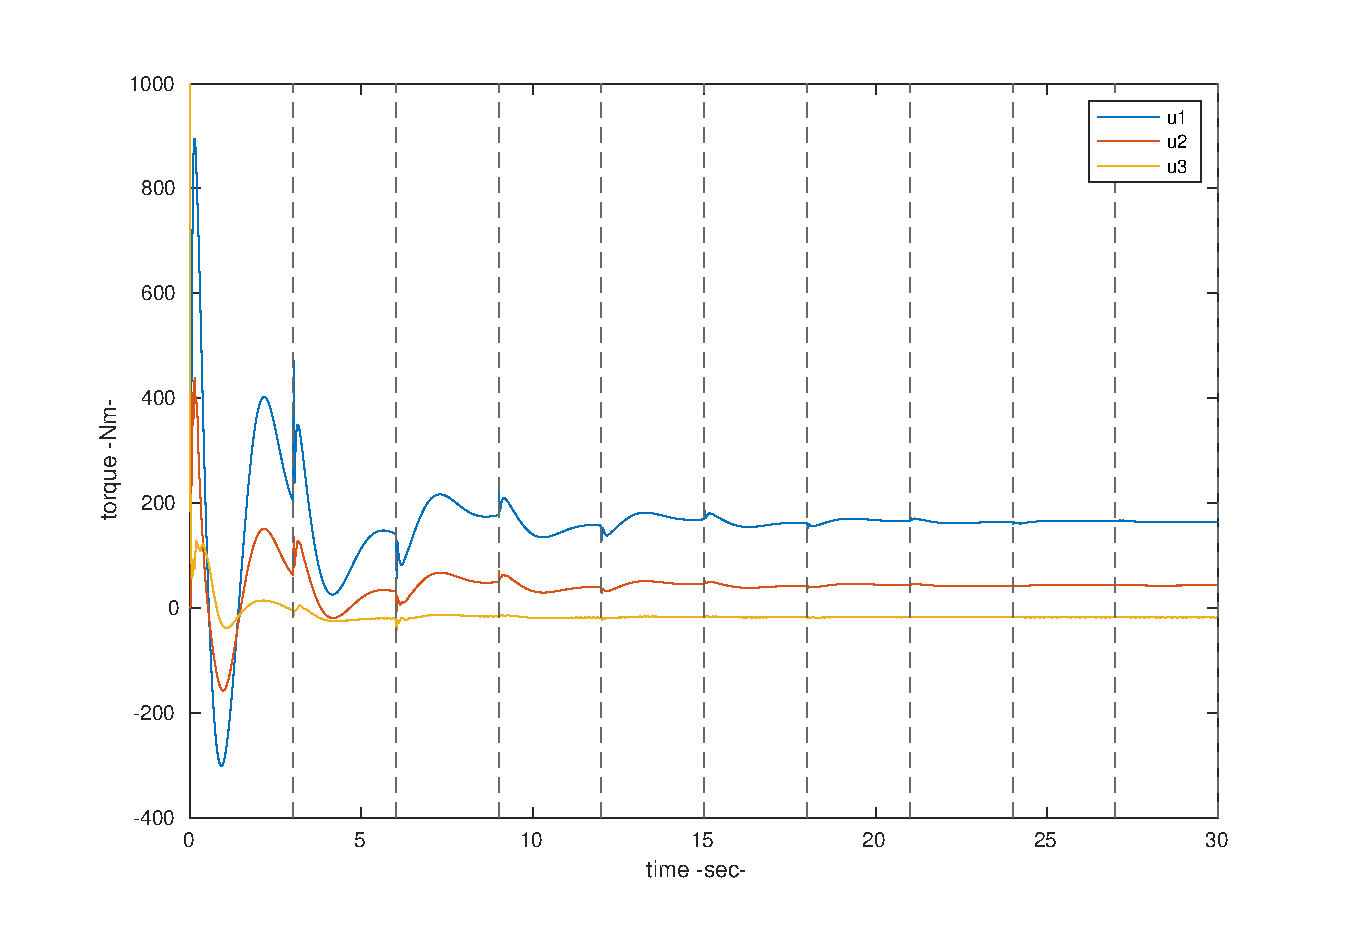
\includegraphics[scale=0.35]{figures/2_1_ceff.eps}
\caption{\label{2_1ceff}
Exp. 2: applied torque.}
\end{minipage}
\hspace{0.5cm}
\begin{minipage}[h!]{0.45\linewidth}
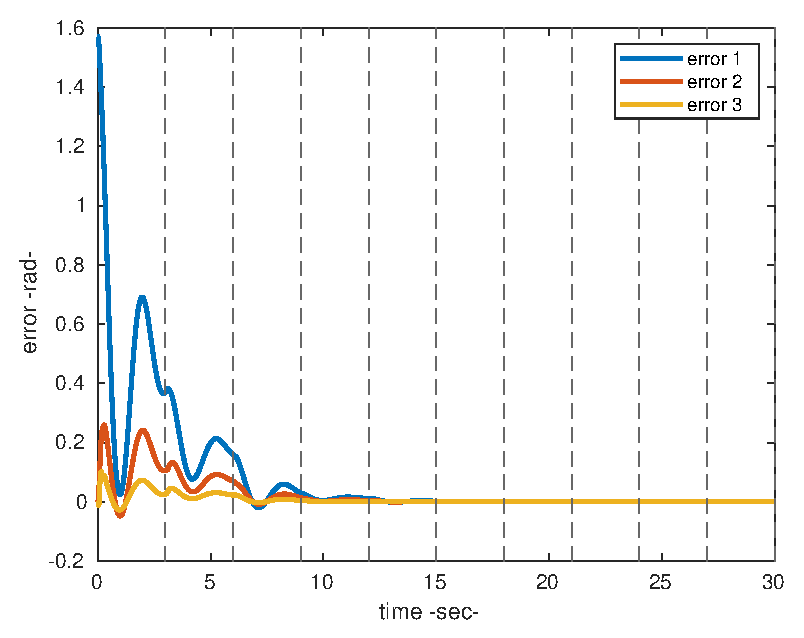
\includegraphics[scale=0.35]{figures/2_2_error.eps}
\caption{\label{2_2err}
Exp. 3: joint level error.}
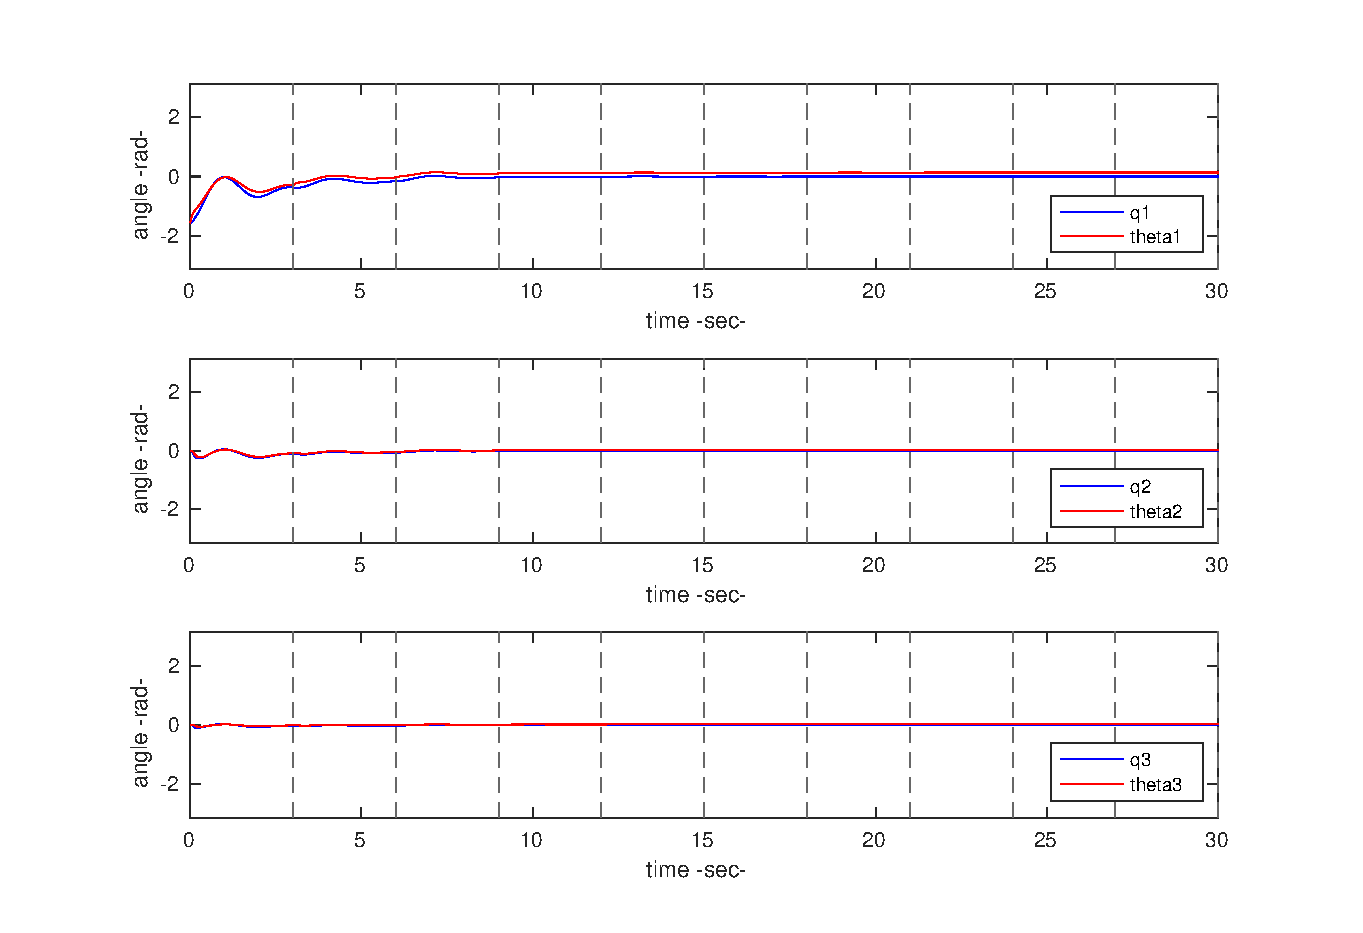
\includegraphics[scale=0.35]{figures/2_2_qtheta.eps}
\caption{\label{2_2qt}
Exp. 3: q and \(\theta\) evolution.}
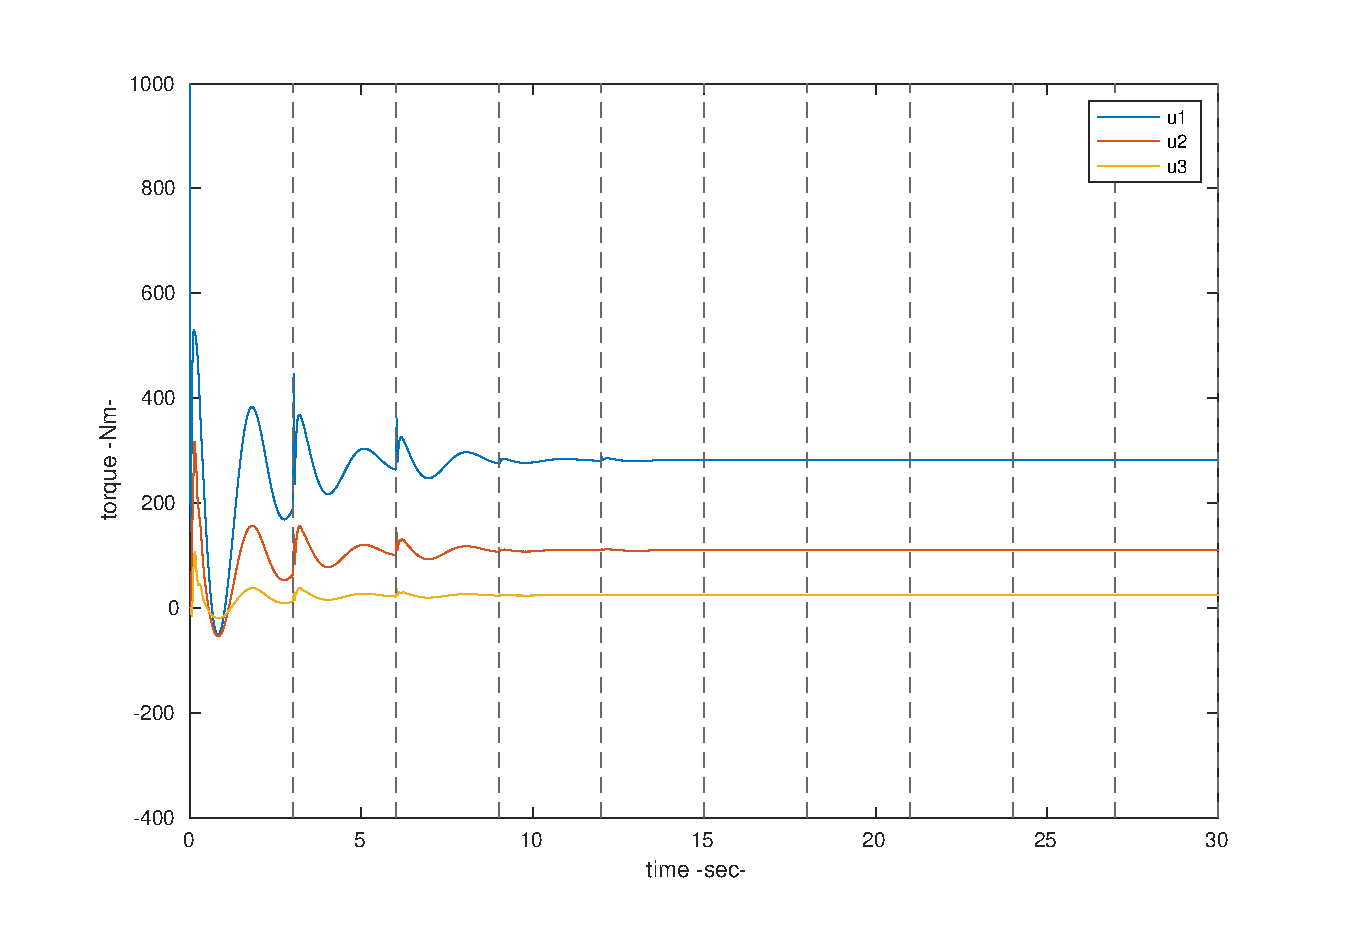
\includegraphics[scale=0.35]{figures/2_2_ceff.eps}
\caption{\label{2_2ceff}
Exp. 3: applied torque.}
\label{fig:assumpt}
\end{minipage}
\end{figure}
\end{center}

\begin{figure}[h!]
\centerline{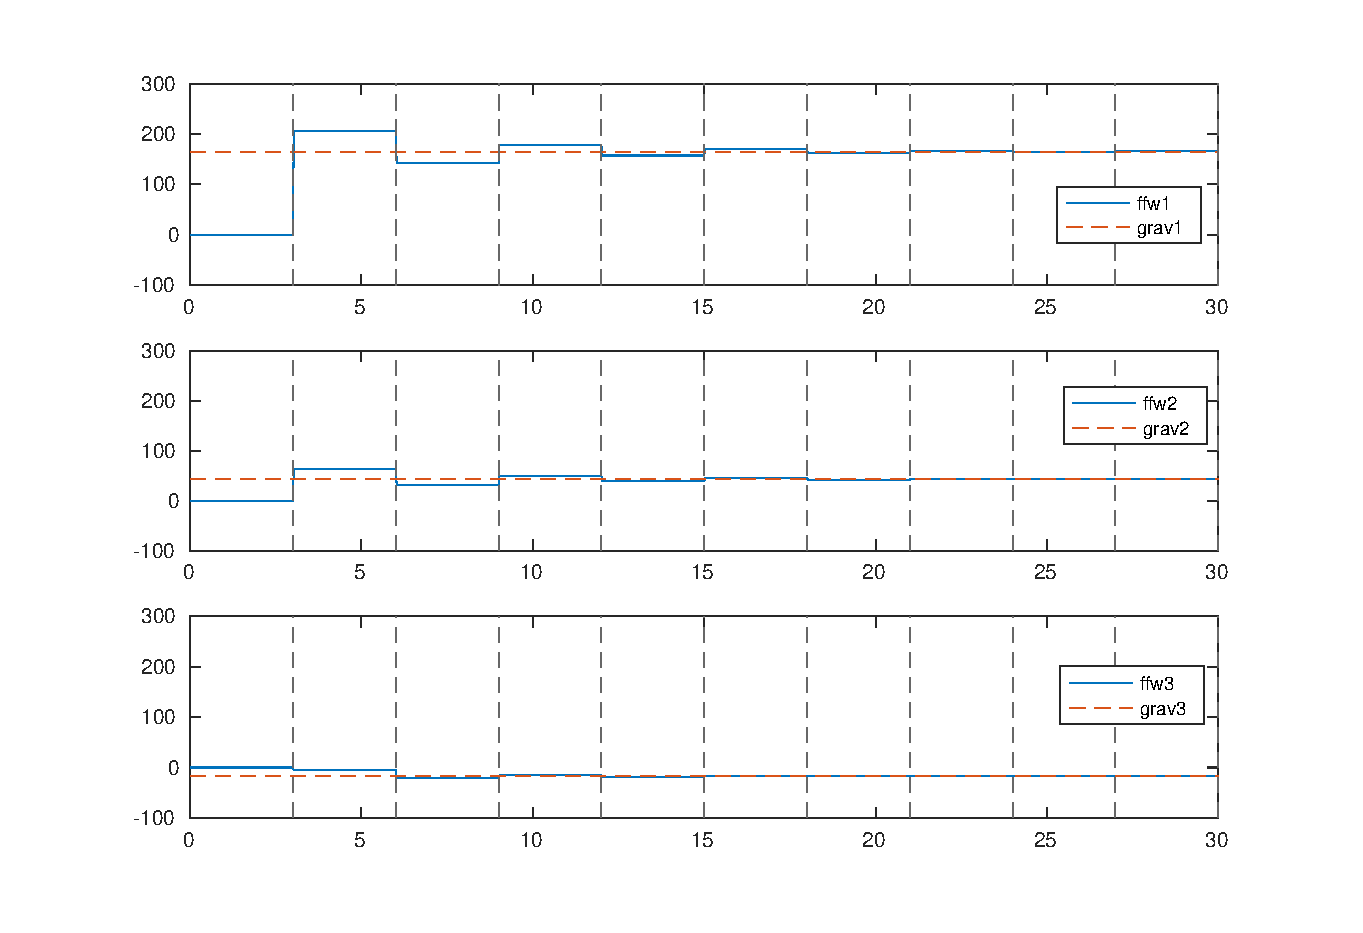
\includegraphics[scale=0.42]{figures/2_1_gravff.eps}}
\caption{\label{2_1gravff}
Experiment 2: evolution of \(u_{t-i}\) w.r.t. \(g(q_d)\).}
\end{figure}

\begin{figure}[h!]
\centerline{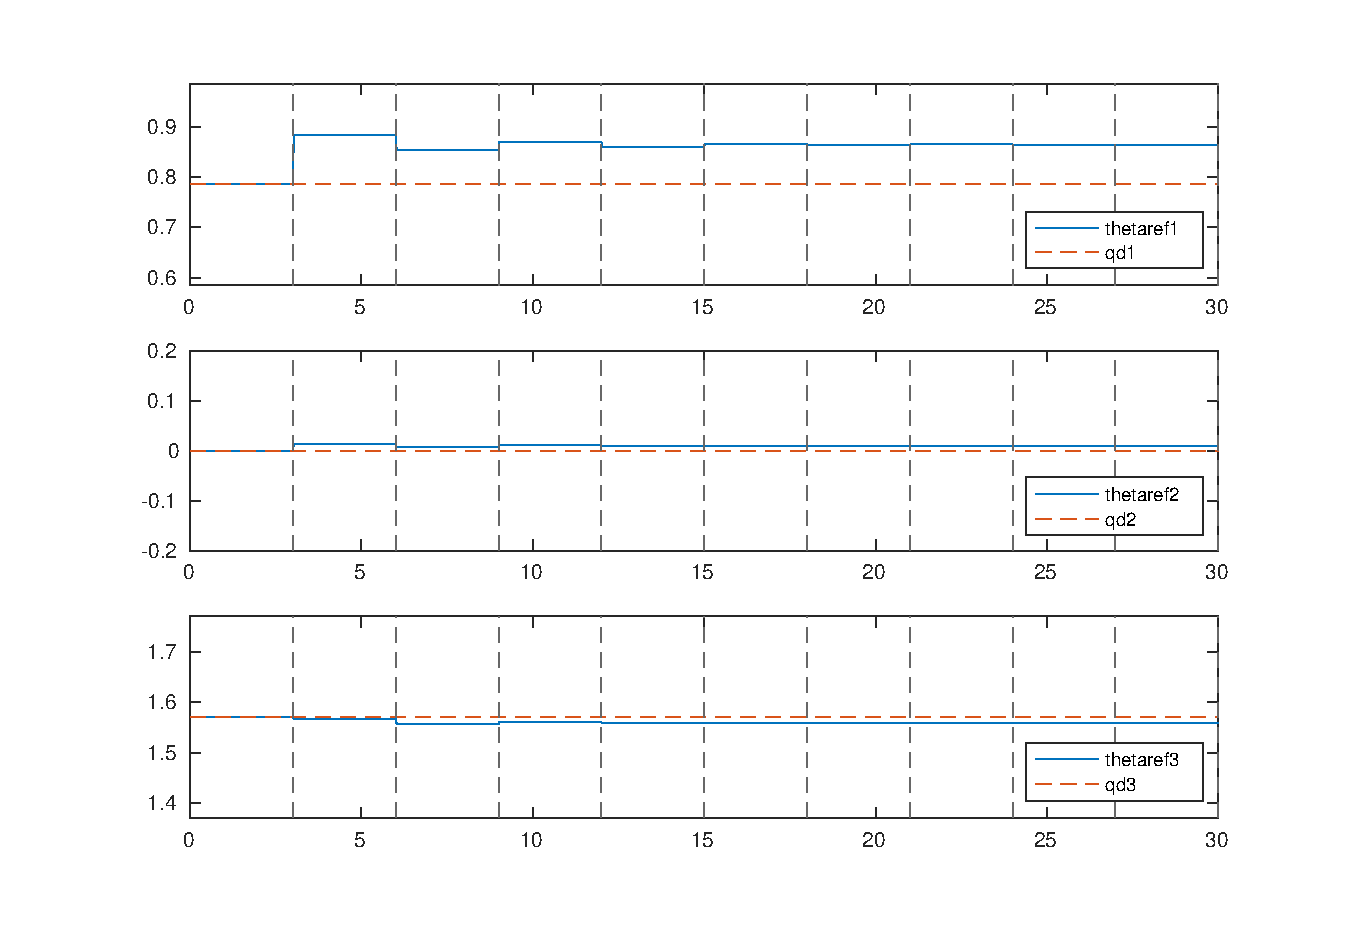
\includegraphics[scale=0.42]{figures/2_1_tqd.eps}}
\caption{\label{2_1tqd}
Experiment 2: evolution of \(\theta_d\) w.r.t. \(q_d\).}
\end{figure}

\begin{figure}[h!]
\centerline{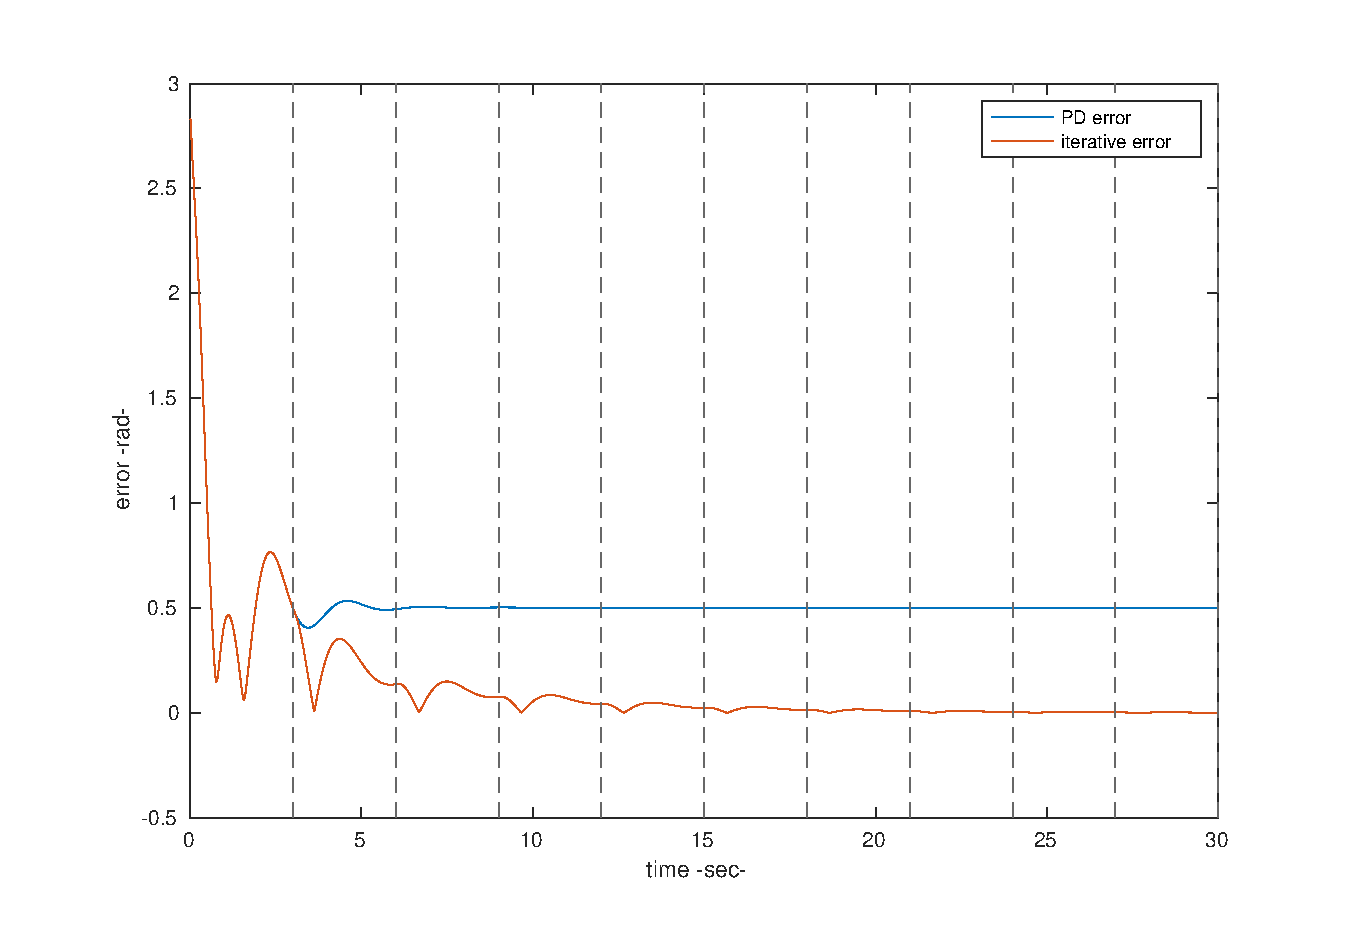
\includegraphics[scale=0.42]{figures/2_1_pdvit.eps}}
\caption{\label{2_1pdvit}
Experiment 2: PD vs Iterative Scheme.}
\end{figure}

\begin{center}
\begin{figure}[h!]
\begin{minipage}[h!]{0.45\linewidth}
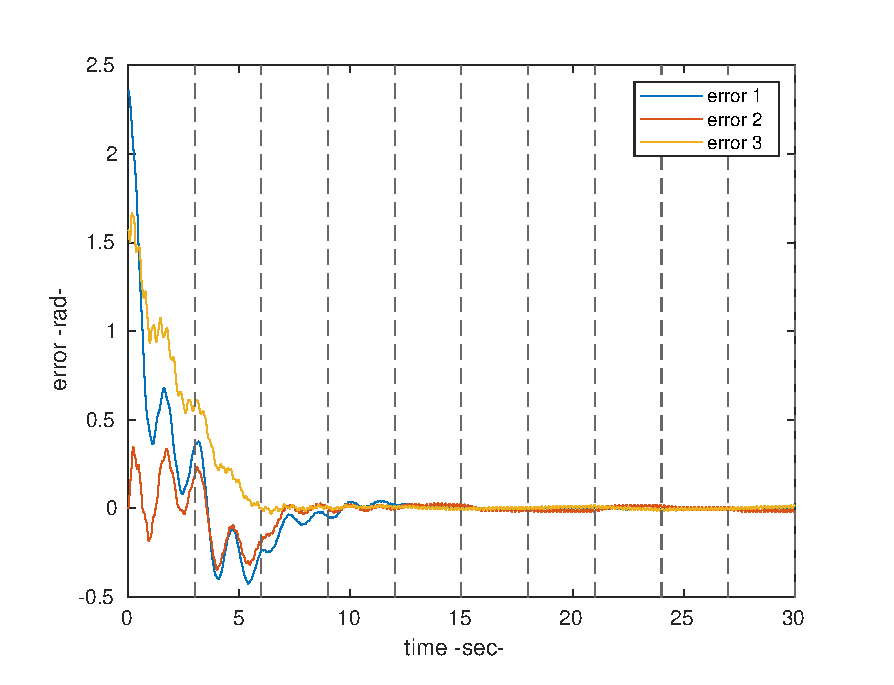
\includegraphics[scale=0.5]{figures/4_lowerrorplot.eps}
\caption{\label{4_e} Exp. 4: joint level error.}
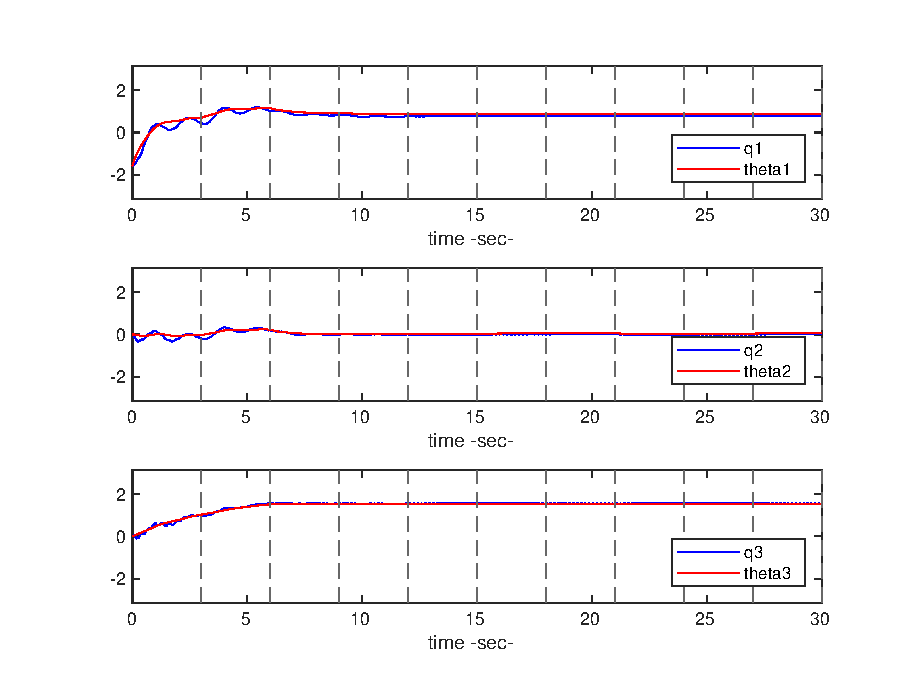
\includegraphics[scale=0.5]{figures/4_lowqthetaplot.eps}
\caption{\label{4_qt}Exp. 4: joint level error.}
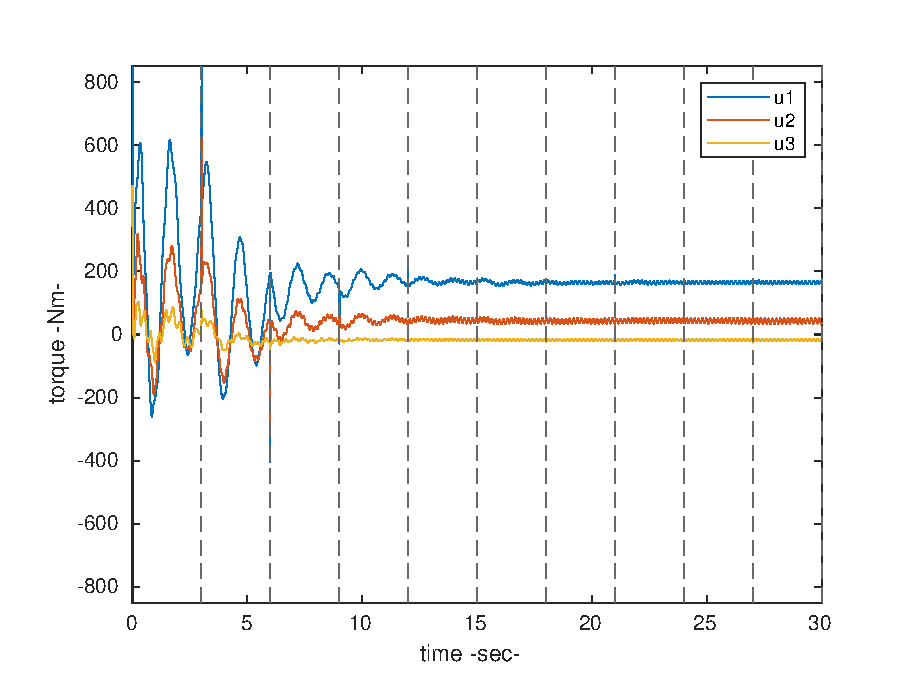
\includegraphics[scale=0.5]{figures/4_loweffortplot.eps}
\caption{\label{4_u}Exp. 4: joint level error.}
\label{fig:ejexample}
\end{minipage}
\hspace{0.5cm}
\begin{minipage}[h!]{0.45\linewidth}
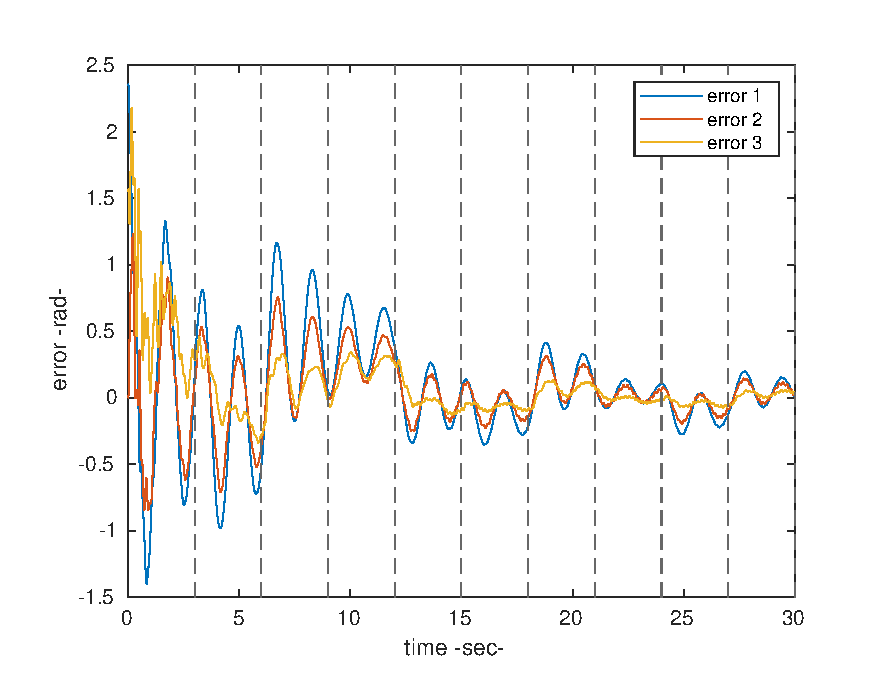
\includegraphics[scale=0.5]{figures/5_lowerrorplot.eps}
\caption{\label{5_e}Exp. 5: joint level error.}
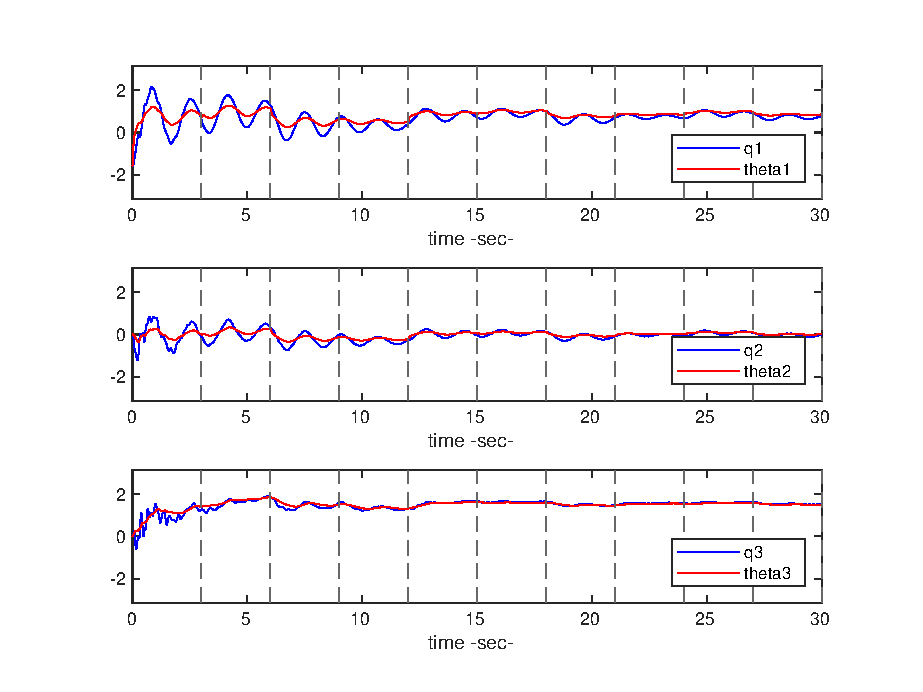
\includegraphics[scale=0.5]{figures/5_lowqthetaplot.eps}
\caption{\label{5_qt}Exp. 5: \(q\) and \(\theta\) evolution.}
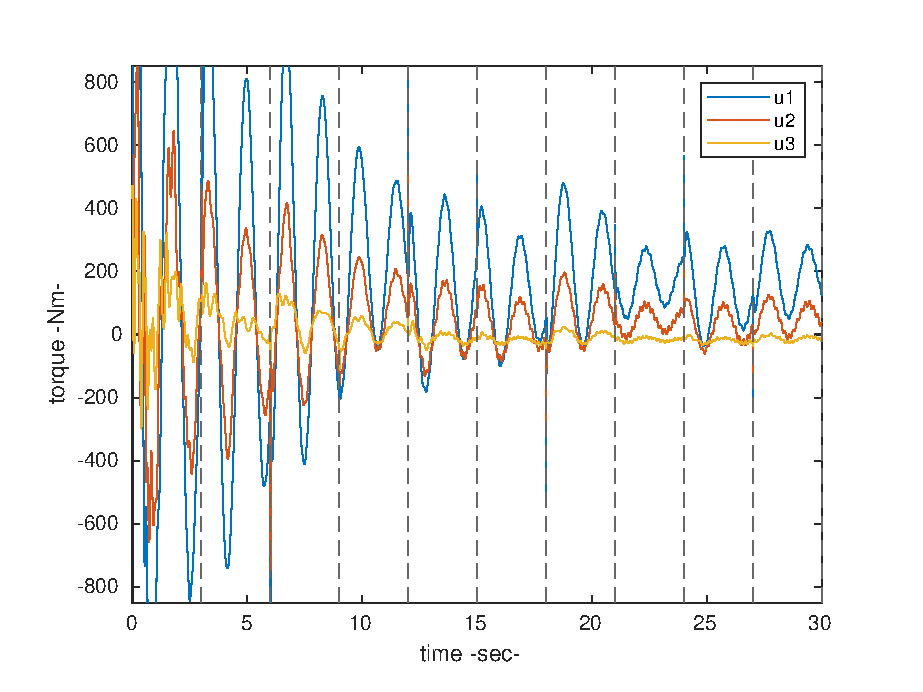
\includegraphics[scale=0.5]{figures/5_loweffortplot.eps}
\caption{\label{5_u}Exp. 5: applied torque.}
\label{fig:assumpt}
\end{minipage}
\end{figure}
\end{center}